\section{Aufbau und Durchf"uhrung}
	\label{sec:durchfuehrung}

	Die Gr"o"sen in Gleichung \eqref{curie} sind durch einfach Mittel nicht zu messen.
	Um auf andere Weise $\chi$ zu bestimmen l"asst sich jedoch die Auswirkung auf ein Magnetfeld einer langen Spule messen.
	Deren Induktivit"at wird ver"andert, wenn man einen paramagnetischen Stoff in die Spule einbringt.

	Mit dem folgenden Aufbau kann die Suszeptibilit"at mittels Messung des Widerstandes $R_\mathrm{P}$ oder der Spannung $U_\mathrm{Br}$ bestimmt werden.

	\begin{figure}[h!]
		\centering
		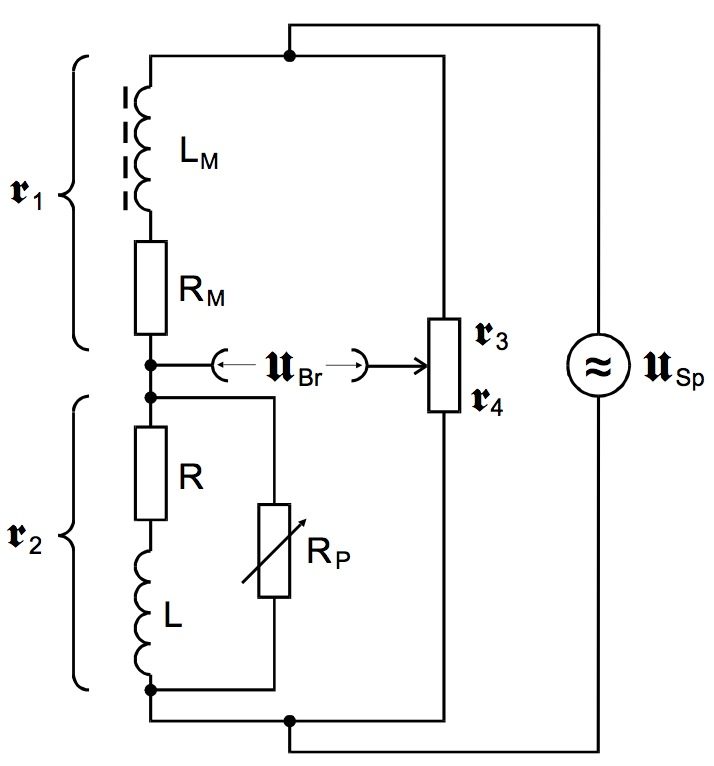
\includegraphics[width = 8cm]{img/aufbau.JPG}
		\caption{Br"uckenschaltung zur Bestimmung der Suszeptibilit"at einiger Stoffe \cite{anleitung}.}
		\label{fig:brueckenschaltung}
	\end{figure}

	\clearpage

	Hier befinden sich zwei m"oglichst identische Spulen, wie gezeigt, hintereinander geschaltet.
	Durch eine "Offnung im Geh"ause des Aufbaus l"asst sich die zu untersuchende Probe in eine der Spulen einbringen.
	Kleine herstellungsbedingte Unterschiede der Spulen k"onnen durch einen variablen Widerstand $R_\mathrm{P}$ ausgeglichen werden.
	Vor jeder Messung muss dieser Widerstand so eingestellt werden, dass die Br"uckenspannung $U_\mathrm{Br}$ minimal wird, beide Spulen also etwa den gleichen Spannungsabfall hervorrufen.

	\subsection{Bestimmung der Suszeptibilit"at durch Messung der Br"uckenspannung}
		\label{subsec:messung_u}
		Nachdem eine Probe in die entsprechende Spule eingebracht wurde, wird die Br"uckenspannung $U_\mathrm{Br}$ gemessen, die direkt Proportional zu $\chi$ ist.
		W"ahlt man eine gro"se Frequenz $\nu$ f"ur die Sinusspannung $U_\mathrm{Sp}$ gilt:

		\begin{eqnarray}
			\nu & \rightarrow & \infty \nonumber \\
			\Rightarrow \quad \chi & = & 4 \frac{F}{A}\frac{U_\mathrm{Br}}{U_\mathrm{Sp}}\,. \label{chi_u}
		\end{eqnarray}

		Mit Kenntnis des Durchmessers $F$ der Spule und des Querschnitts $A$ der Probe kann damit durch Messung der Spannungen $U_\mathrm{Br}$ und $U_\mathrm{Sp}$ die Suszeptibilit"at $\chi$ berechnet werden.

	
	\subsection{Bestimmung der Suszeptibilit"at durch Messung des Regelwiderstandes}
		\label{subsec:messung_u}
		Die Br"uckenspannung $U_\mathrm{Br}$, die sich nach dem Einschieben einer Probe ergeben, hat kann nun erneut durch Variation des Widerstandes $R_\mathrm{P}$ minimiert werden.
		Dabei ist $\chi$ ebenfalls proportional zum Unterschied $\Delta R$ der Widerst"ande vorher und nachher und l"asst sich durch die Messung dieser bestimmen:

		\begin{equation}
			\label{chi_r}
			\chi = 2 \frac{\Delta R}{R_3}\frac{F}{A}\,.
		\end{equation}

	\subsection{Unterdr"uckung der St"orspannung}
		Die Spannungen dieser Messungen liegen im Nanovoltbereich und werden daher leicht durch "au"sere Einfl"usse verf"alscht.
		Da die Br"uckenschaltung in diesem Versuch aber mit einer Sinusspannung $U_\mathrm{ein}$ konstanter Frequenz gespeist wird, kann ein Selektivverst"arker die St"orspannungen herausfiltern.

		Um die Qualit"at dieses Filters zu beurteilen, muss dessen G"ute $Q$ bestimmt werden.
		Daf"ur werden mit einer Eingangsspannung $U_\mathrm{ein}$ konstanter Amplitude Signale unterschiedlicher Frequenz $\nu$ hinter dem Selektivverst"arker gemessen.
		Das Verh"altnis $V$ der gemessenen Spannung $U_\mathrm{aus}$ zur Eingangsspannung $U_\mathrm{ein}$ nimmt bei einer bestimmten Frequenz - der Durchlassfrequenz $\nu_0$ - etwa den Wert 1 an.
		Mit den Frequenzen $\nu_+$ und $\nu_-$, an denen das Verh"altnis $V$ gerade $1/\sqrt{2}$ betr"agt, l"asst sich die G"ute bestimmen und es gilt

		\begin{equation}
			Q = \frac{\nu_0}{\nu_+ - \nu_-}\,. \label{Gleichung:Guete}
		\end{equation}

		Bei dieser Messung sollten alle Verst"arker deaktiviert sein.

		Bei den Messungen mit aktivierten Verst"arkern ist es wichtig, den genauen Verst"arkungsgrad zu bestimmen.
		Dazu wird bei eingeschalteten Verst"arkern $V$ erneut berechnet.
		Alle gemessenen Spannungen werden dann um diesen Faktor bereinigt.